\documentclass{trkut}% Reaalkooli vormistus. Muidu "report" või "article".
\usepackage[style=trkut]{biblatex}% Kasutatud kirjanduse genereerimine
\usepackage{pgfplots}
\usepackage{amsmath}
\usepackage{siunitx}
\addbibresource{viited_eesnimi_perekonnanimi.bib}% Viidete info fail
\defbibheading{bibliography}{\addchap{#1}}% Lisame kasutatud materjalid sisukorda

\pealkiri{Atmosfääri mudeldamine ja katseandmete põhjal täpseima mudeli leidmine} % Kahel real
\autor{Jarl Patrick Paide}
\klass{11.a}
\juhendaja{õp Mart Kuurme } %\\ õp Kaarel Kivisalu}% Toetab praegu ainult ühte juhendajat, manual fix: muuda cls failis juhendaja -> juhendajad

\begin{document}
\maketitle% Tiitelleht
\tableofcontents% Sisukord

\addchap{Sissejuhatus}
\nummerdame% See käsk peab olema kohe peale sissejuhatust
%See teema on aktuaalne, kuna see on väga huvitav ja ma tahan seda uurida...
Globaliseeruvas ja ülerahvastatud maailmas on atmosfääri reostatus üks kõige olulisemaid probleeme. Atmosfääri reostusega kaasneb kasvuhooneefekt - kliima soojenemine, mis omakorda viib maailmamere tõusule. Atmosfääri mudeldamine aitab mõista atmosfääris toimuvaid protsesse ja leida lahendusi atmosfääri seisundi arendamiseks. Mudeli andmeid saab kasutada globaalse atmosfääri mudeli arendamisel.

Uurimistöö eesmärk on leida vaatlusandmete alusel võimalikult täpne mudel, mis kirjeldaks atmosfääri temperatuuri ja rõhu seoseid vastavalt kõrgusele maapinnast. Uurimisküsimus on "Millised seosed on atmosfääris mõõdetavate parameetrite vahel - temperatuur, rõhk ja kõrgus maapinnast?".

Uurimistöö alguses leitakse erinevate eeldustega erinevad seosed temperatuuri ja rõhu sõltuvusest kõrgusest. Praktilises osas tehakse mõõtmisi heeliumõhupalli külge kinnitatud mõõteriistaga, mis lennutatakse stratosfäärini ja pärast kontrollitakse katseandmete põhjal teoreetilises osas saadud seoste kehtivust.





\chapter{Teooria}
Teooria osas proovitakse leida erinevaid täpseid viise, kuidas kirjeldada rõhu ja temperatuuri sõltuvust kõrgusest.

\begin{figure}[h]
	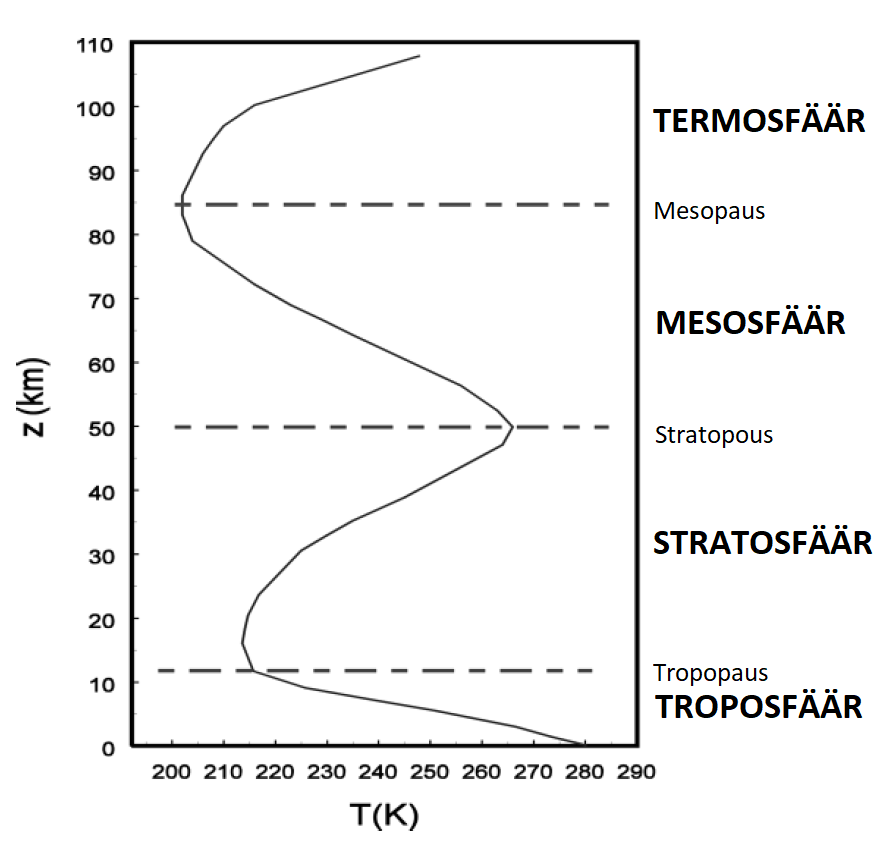
\includegraphics[width=0.5\textwidth]{PicGra/Profile2.png}
	\caption{Temperatuuri sõltuvus kõrgusest}
	%\allikas{Minu programm}
	\label{profile}% Selle järgi viidatakse, see rida peab olema pärast \caption
\end{figure}

Joonisel \ref{profile} on näha, kuidas temperatuur muutub kõrguse kasvades. Troposfääris temperatuur langeb ja stratosfääris temperatuur tõuseb. Kõrguse kasvades rõhk väheneb, sest kõrguse kasvades väheneb ülevalpool oleva õhu mass, mis surub õhku kokku tekitades rõhku. Kuna rõhk väheneb, siis temperatuur langeb. See seletab temperatuuri langust troposfääris. Peale troposfääri tuleb osoonikiht, mis asub stratosfääris. Osoon neelab päikeselt tulevat kiirgust muutes selle soojuseks. Mida kõrgemal, seda vähem kiirgust on neelatud päikese poolt ja seda soojem. Eelkirjeldatud atmosfääri kihtides on kogutud käesoleva uurimistöö katseandmed.

Selles peatükis on avaldatud temperatuuri ja rõhu sõltuvused kõrgusest erinevate meetoditega, otsides kõige täpsemat seost.

Termodünaamika esimene seadus on avaldatud alljärgnevalt
\begin{equation}\label{eq1}
dU = dQ - dA
\end{equation}
kus $dU$ on gaasi siseenergia muutus, $dQ$ on soojushulga muutus ja $dA$ on töö muutus.

Gaasi siseenergia $U$ avaldub vabadusastmete $i$ kaudu järgneva seose abil
\begin{equation}\label{eq5}
U = \frac{i}{2} \nu R T
\end{equation}
Konstantse ruumala puhul tööd ei tehta, seega kogu soojus läheb siseenergia suurendamiseks. Saame soojusmahutavuse, võttes siseenergia muudust tuletise temeratuuri järgi.
\begin{equation}\label{eq6}
C_V = \frac{dQ}{dT}=\frac{i}{2}\nu R
\end{equation}
Molaarset soojusmahutavust saab avaldada valemiga $c_V = \frac{C_V}{\nu}$ saades molaarseks soojusmahutavuseks
\begin{equation}\label{eq7}
c_V = \frac{i}{2}R
\end{equation}

Kui aga vaadata isobaarilist protsessi, siis vaadates olekuvõrrandit tuleneb $pdV=\nu RdT$, ning gaas teeb tööd $dA = pdV = \nu RdT$. Avaldades need valemisse \ref{eq1} saame
\begin{equation*}
dQ = dU + dA = \frac{i+2}{2} \nu R dT
\end{equation*}
millest järeldub
\begin{equation*}
c_p=\frac{i+2}{2}R
\end{equation*}
Samuti saab näidata $c_V$ ja $c_p$ vahelist seost
\begin{equation}\label{eq9}
c_p = c_V + R
\end{equation}

Vaatame õhukest õhuriba laiusega $dz$ kõrgusel $z$. Rõhu muutust kõrguste $z$ ja $z + dz$ vahel saab kirjeldada valemiga
\begin{equation}\label{eq10}
dp=-\rho (z) gdz
\end{equation}
Kui seda integreerida, siis saab kätte rõhu muutuse sõltuvalt kõrgusest. Aga kuna tihedus ei ole konstantne, siis on vaja kõigepealt leida kuidas tihedus muutub kõrguse muutumisega.

\section{Ideaalne gaas}
On olemas erinevaid gaasi mudeleid. Nendest kõige tuntum on ideaalse gaasi olekuvõrrand. Ideaalne gaas erineb reaalsest gaasist kahe eelnuse poolest. Ideaalses gaasis ei arvestatta osakeste vahelist vastastikjõude. Ideaalses gaasis on osakestel tühiselt väike suurus. Võib eeldada, et gaas on ideaalne siis kui rõhk on väike kriitilise rõhu suhtes ja temperatuur on kõrge kriitilise temperatuuri suhtes. Kui rõhk on kõrge siis on osakeste vahelisi kokkupõrkeid palju ja osakeste suurus saab oluliseks. Kui temperatuur on madal siis liiguvad osakesed aeglaselt ja osakestel on rohkem aega olla üksteise mõjuväljas ja saada mõjutatud. Kui me vaatame atmosfääri siis kõige kõrgem rõhk on maa lähedal ja kõrguse tõustes see väheneb, millega väheneb ka osakeste vaheline vastasmõju. Atmosfääris olevad rõhud on väikesed võrreldes õhu kriitilise rõhuga. Temperatuur võib langeda atmosfääris küll madalale, aga mitte piisavalt madalale, et see läheneks kriitilisele temperatuurile. Seega võib eeldada, et atmosfääris olevad gaasid käituvad kui ideaalsed gaasid.

Sellisel juhul saame kasutada ideaalse gaasi olekuvõrrandit
\begin{equation}\label{eq8}
PV=\nu RT
\end{equation}

\subsection{Isotermiline atmosfäär}
Oletame, et armosfääris on kõikjal ühtlane temperatuur. Sellisel juhul on atmosfäär isotermiline ja me saame asendada valemi \ref{eq8} valemise \ref{eq10} saades järgmise seose
\begin{equation}\label{eq16}
\frac{dp}{p} = -\frac{\mu g}{RT}dz
\end{equation}
Kuna temperatuur on konstantne, siis on ka $\frac{\mu g}{RT}$ konstantne ning seda integreerides saame järgneva
\begin{equation*}
\int_{p_0}^{p} \frac{dp}{p}  = \int_{0}^{z} -\frac{\mu g}{RT}dz
\end{equation*}
\begin{equation*}
\ln(\frac{p}{p_0}) = - \frac{\mu g}{RT} z
\end{equation*}
Kus $T$ on atmosfääri konstatntne temparatuur, $z$ on kõrgus maapinnalt, $p_0$ on kõrgus maapinnalt ja $p$ on rõhk kõrgusel $z$ maapinnast ja $p$ sõltub kõrgusest järgnevalt
\begin{equation*}
p = p_0 e^{-\frac{\mu g}{RT}z}
\end{equation*}
Kuid see valem ei kehti, sest atmosfääris pole ühtlane temperatuur.

          
\subsection{Adiabaatiline atmosfäär}
Adiabaatiline protsess on termodünaamiline protsess, mille käigus ei toimus soojusvahetust väliskeskkonnaga.

Harilikult on õhumassid atmosfääris tugevas liikumises, nii et nad liiguvad pidevalt üles-alla. Kuna kõrgemal on rõhk väiksem kui all, siis jahtub gaas üles liikudes adiabaatilise paisumise tõttu (õhumasside suurte mõõtmete tõttu on soojusjuhtivus hästi aeglane).

Kuna adiabaatilises protsessis soojusvahetust ei toimu, siis valemis \ref{eq1} $dQ=0$. Gaasi poolt tehtud töö on $d A=pdV$ ja gaasi siseenergia muut on $dU=\nu c_VdT$. Sellest järeldub
\begin{equation}\label{eq2}
\nu c_VdT = -pdV
\end{equation}
Ideaalse gaasi olekuvõrrandist \ref{eq8} saame tuletist võttes ja avaldades järgneva
\begin{equation}\label{eq3}
dT = \frac{pdV+Vdp}{\nu R}
\end{equation}
Asendades \ref{eq3} valemi valemisse \ref{eq2} saame uue seose
\begin{equation}\label{eq4}
pdV(c_V+R)+c_VVdp=0
\end{equation}
Asendame siia sisse valemi \ref{eq9} ja adiabaadi näitaja
\begin{equation*}
\gamma \equiv \frac{c_p}{c_V}
\end{equation*}
Nüüd eelmisi seoseid kasutades ja ümber paigudades saame võrrandi
\begin{equation*}
\gamma \frac{dV}{V} + \frac{dp}{p} = 0
\end{equation*}
Seda integreerides saame
\begin{equation*}
 \int \gamma \frac{dV}{V} + \frac{dp}{p} = \gamma \ln(V) + \ln(p) = Const.
\end{equation*}
Sellest saame järeldada
\begin{equation*}
pV^\gamma = Const.
\end{equation*}
Samuti kasutades ideaalse gaasi olekuvõrrandid saame tuletada veel 2 seost
\begin{equation}\label{eq13}
p^{1-\gamma}T^\gamma = Const.
\end{equation}
\begin{equation*}
V^{\gamma-1}T = Const.
\end{equation*}
Valemist \ref{eq13} saame
\begin{equation*}
d\ln(p^{1-\gamma}T^\gamma) = 0
\end{equation*}
Millest saame
\begin{equation}\label{eq17}
\frac{dp}{p} = \frac{\gamma}{\gamma-1}\frac{dT}{T}
\end{equation}
Võttes nüüd valemi \ref{eq16} ja valemi \ref{eq17}
\begin{equation*}
\frac{dT}{dz}=-\frac{\gamma-1}{\gamma} \frac{\mu g}{R}
\end{equation*}
Seda integreerides saame
\begin{equation*}
\int_{T_0}^{T} dT = \int_{0}^{z} -\frac{\gamma-1}{\gamma} \frac{\mu g}{R} dz
\end{equation*}
\begin{equation*}
T - T_0 = - \frac{\gamma - 1}{\gamma} \frac{\mu g}{R} z
\end{equation*}
Kus $T_0$ on temperatuur maapinnal ja $T$ on temperatuur kõrgusel $z$, mille saab avaldada sõltuvusena
\begin{equation*}
T=T_0 \bigg( 1-\frac{\gamma-1}{\gamma} \frac{\mu g}{R T_0} z \bigg)
\end{equation*}
Kasutades nuud seost \ref{eq13} saame seose
\begin{equation*}
p = p_0 \bigg( 1-\frac{\gamma-1}{\gamma} \frac{z}{z_0} \bigg)^\frac{\gamma}{\gamma-1}
\end{equation*}


\section{Virtuaalne temperatuur}


\chapter{Katse ülesehitus}
Katse käigus mõõdeti atmosfääris, troposfääris ja stratosfääri madalametes kihtides, rõhku, temperatuuti ja õhuniiskust. Selle jaoks kasutati heeliumõhupalli külge kinnitatud sondi, mis tegi mõõtmisi.

Andmeid kogutakse heeliumiga täidetud õhupalliga kaasa saadetud sondiga, mis mõõdab erinevaid andmeid. Põhilisteks andmeteks on kõrgus, asukoht, aeg, välistemperatuur ja rõhk. Sondi pardal on Raspberry Pi arvuti. Õhupall kerkib atmosfääri kõrgemadesse kihtidesse, sest üleslükkejõud ületab kerge gaasi ja sondi massi. Kõrgemale tõustes rõhk väheneb. Et õhupalli siserõhk oleks tasakaalus välisrõhuga, suureneb õhupalli ruumala, kuni õhupall lõhkeb ülepingest. Peale seda kukkub sond alla ja leitakse GPS'ga üles.

\section{Katsemetoodika valik}
Selles uurimistöös tehtud katsed on tehtud koostöös Eesti kosmosekoolide võrgustikuga.

Eesti kosmosekoolide võrgustik oli enne selle uurimistööga tehtud lendu teinud kaks lendu. Esimene lend mis tehti 29. märtsil kestis umbes kaks tundi, kus kõrgeim punkt milleni jõuti oli 26474 m. Selleks läks aega poolteist tundi. Kokku tehti 220 mõõtmist. Mõõtmise alla kuulusid kellaaeg, laiuskraad, pikkuskraad, kõrgus, kapsli sisetemperatuur, välistemperatuur ja rõhk. Teine lend tehti 11. mail ning seekord kestis lend peaaegu neli tundi, jõudes kolme ja poole tunniga kõrgusele 32608 m. Katse tegijad muutsid õhupallis heeliumi kogust, mille tõttu oli tõusmise kiirus väiksem, aga õhupall plahvatas hiljem ja jõuti kõrgemale. Seekord tehti 4300 mõõtmist ja mõõdeti samu parameetreid.

Katse korraldamiseks ja läbiviimiseks vajalikud oskused saadi Eesti kosmosekoolide võrgustiku poolt korraldatavast koolituselt ja sealt on pärit vastav metootika.

Selle uurimistöö käigus tehti katse milleks oli heeliumõhupalliga andmete kogumine kogu lennu vältel. Heeliumõhupalli külge kinnitati sond, mis mõõtis õhurõhku, temperatuuri, õhuniiskust ja asukohta. Lend koraldati 10. veebruaril 2019.

\section{Katse planeerimine}
Alguses oli plaanis lend teha väätsa staadionilt, aga kasutades http://predict.habhub.org/ lehel olevat kalkulaatorit oli ennustusest näha, et sond oleks kukkunud jõhvi lähedale. Kuna eksimusruum võib olla suur ning Venemaa piir ja meri pole kukkumis kohast kaugel otsustatti lennu start teha võimalikult edelast, nii et edela tuultega kalduks sond Kesk-Eestisse. Rihtides lõppsihtkohta Paide peale otsustatti start teha Varblast, Pärnumaalt.

Lennu jaoks oli vajalik saada lennuametilt kooskõlastus.

Sondi ehitamise eest vastutasid Tallinna Reaalkooli põhikooli õpilaste robootikameeskond Viirus. Sondi põhiehitusmaterjaliks oli penoplast ja puidust tikkud. Sond pidi hoidma sisetemperatuuri madalate välistemperatuuri eesti, et sisemuses olev elektroonika töötaks. Sammuti peab korpus vastu pidama kukkumisele, ning kõige juures peab olema korpus võimalikult kerge. Selle tõttu valiti korpuse materjaliks penoplast ja tikkud. Kuna ühe lennuga saab üles saata mitu katset siis otsustasid põhikooli õpilaste meeskond Viirus koguda atmosföörist tolmu tõmmates õhku läbi filtri. 

Sondi sees olev ruum oli jaotatud kaheks. Alumises olid kaks toru mis olid parralleelsed ja läbisid sondi kere. Nenede sees olid klappid, ventilaator ja filtrid. Selle eesmärgiks oli koguda tolmu ja muud, mis jääb filtrisse kinni kõrgemal kui 20km. Teatud kõrguse saavutamisel pöörab raspbarry Pi mootori \SI{90}{\degree} päripäeva avades nii klappid ja sulgedes lüliti. mille tõttu hakkavad ventilaarotid tööle. Kui võrgus on vähenenud soovitud kõrgusest siis pöörab raspbarry Pi mootori algasendisse. Sulgedes sellega klappid ja ühendades ventilaarotid vooluringist lahti. Tolmu kogumine ei käi selle uurimistöö juurde.

\begin{figure}[h]
	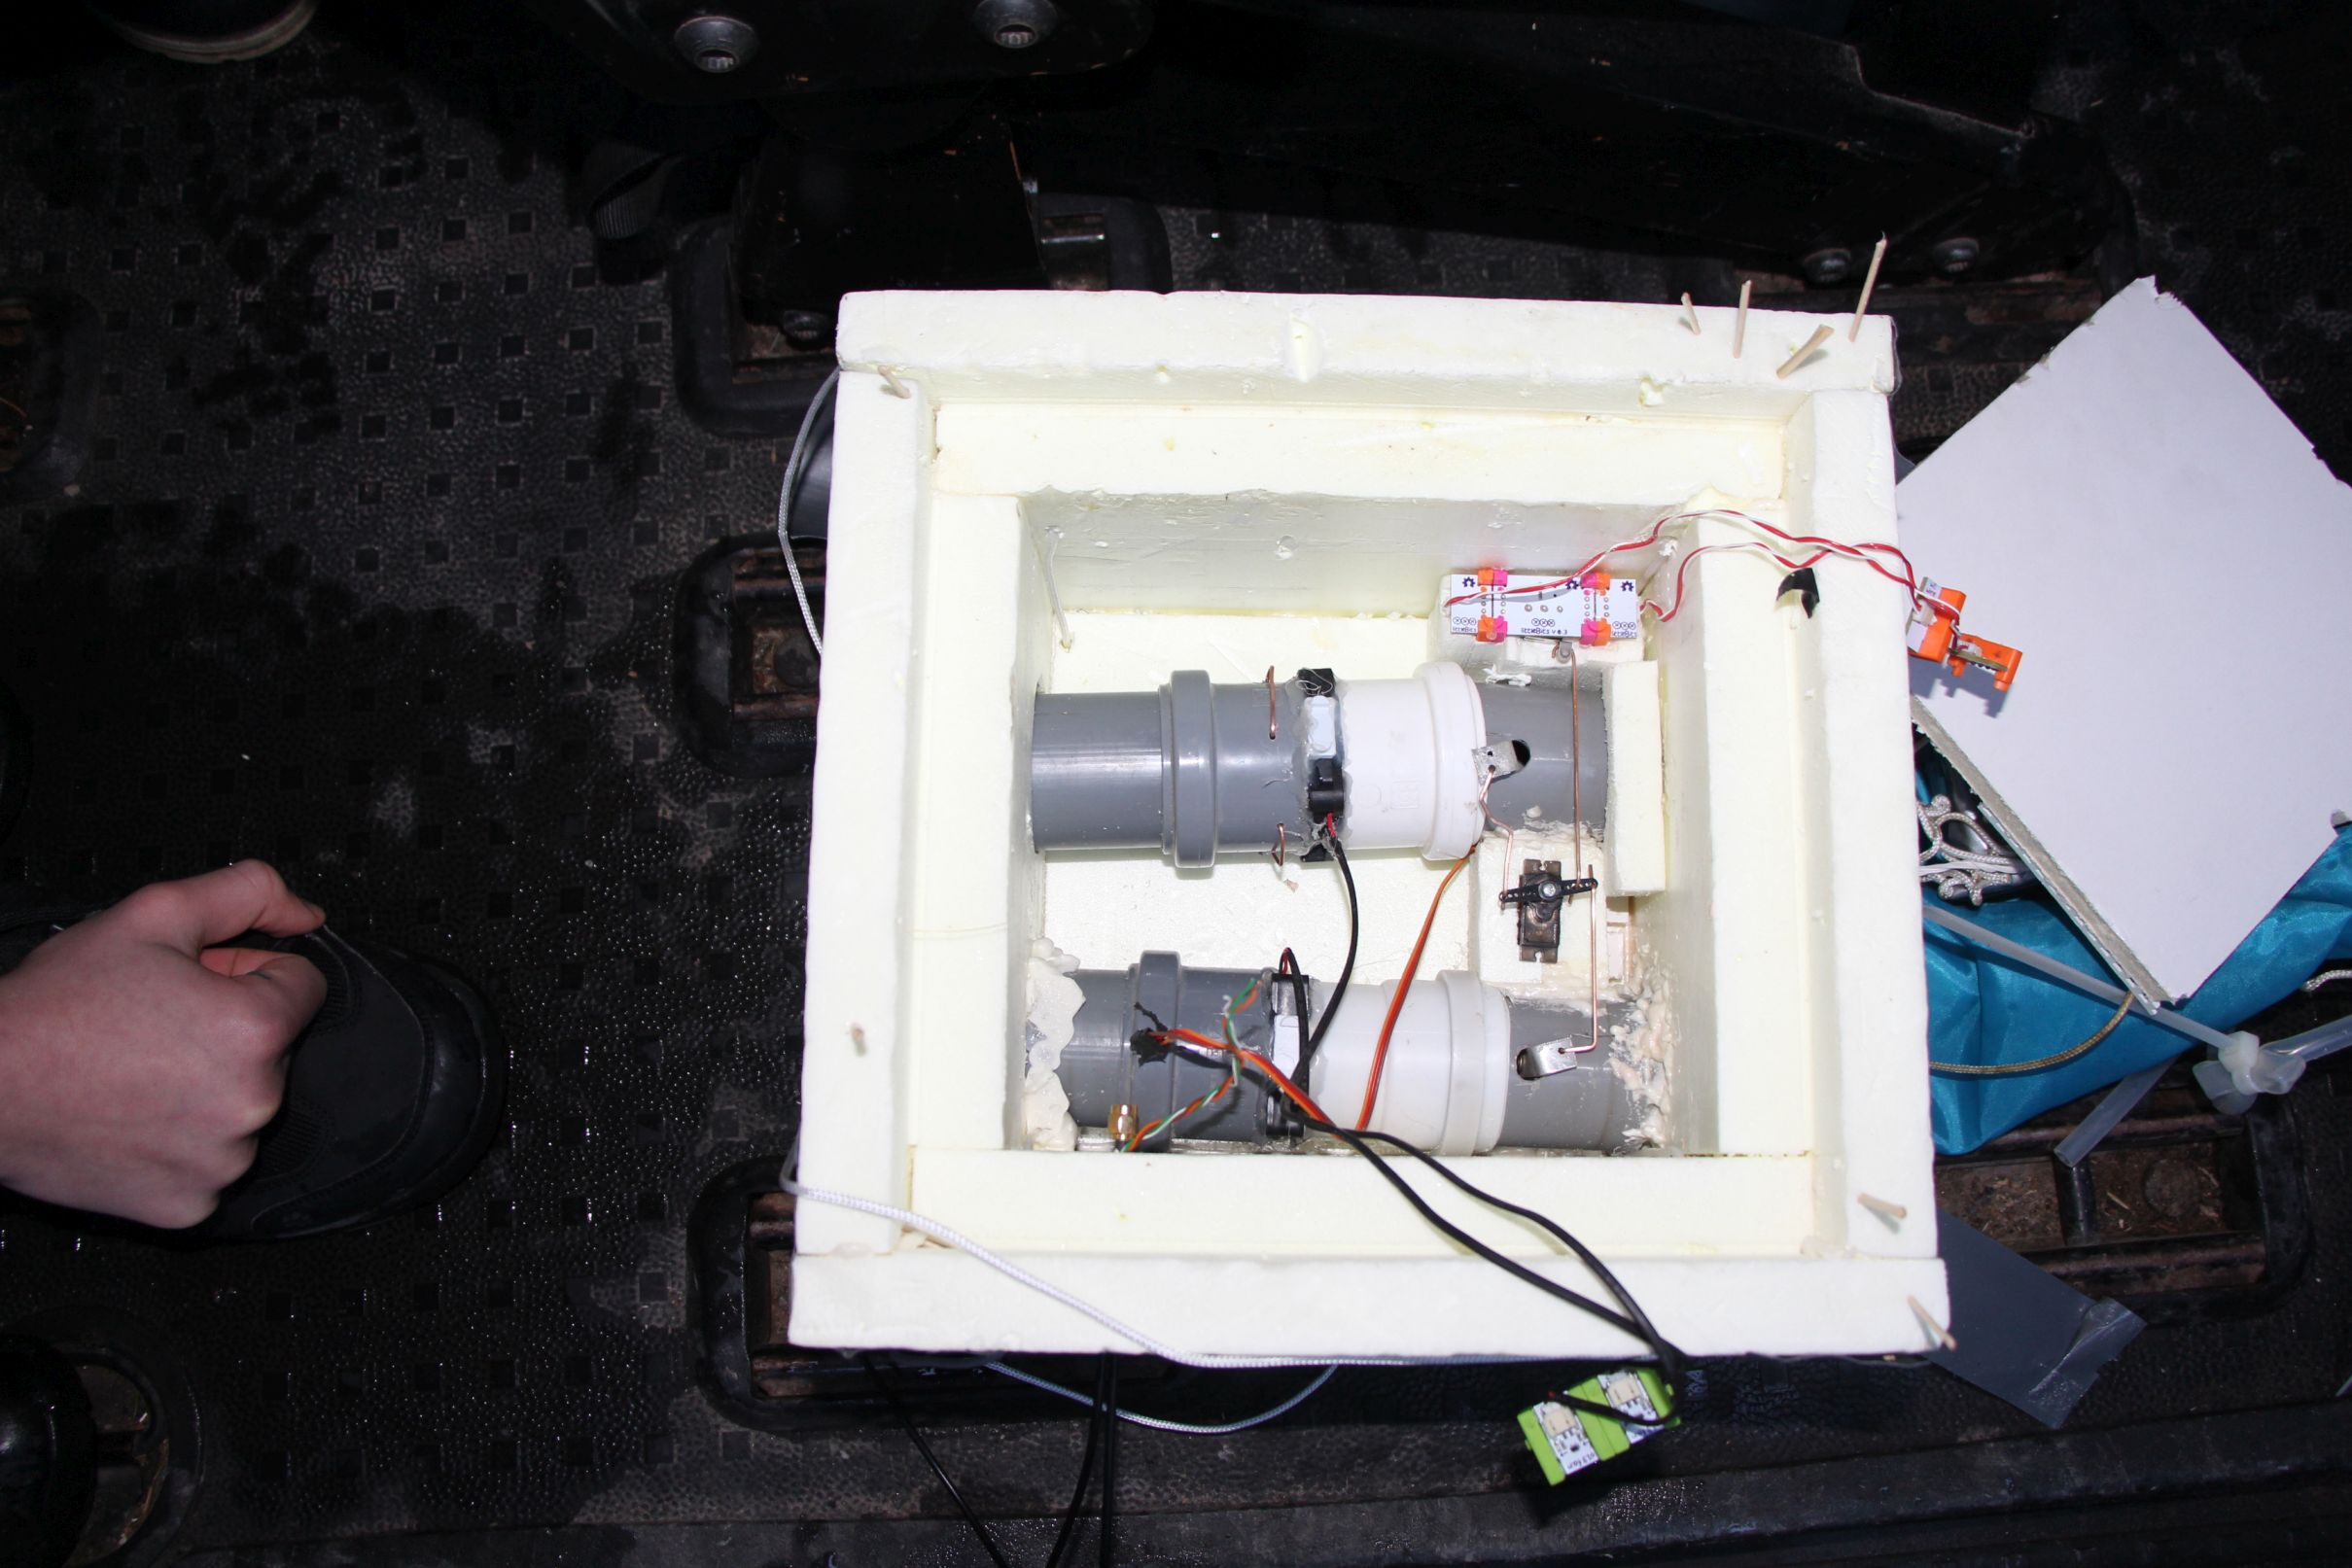
\includegraphics[width=0.5\textwidth]{PicGra/sond2korrus.jpg}
	\caption{Pilt sondist}
	\allikas{\url{http://pildid.real.edu.ee/main.php?g2_itemId=84949}}
	\label{sond}
\end{figure}

Ülemises osas oli kogu tehnika. Mõõtmisi tegi ja klappe avas Raspberry Pi arvuti. Voolu andis nii ventilaatoritele kui ka Raspberry Pi'le akkupank. Raspberry Pi külge oli kinnitatud raadio antenn, Gps antenn mootor klappide jaoks ja andur BME280 mis mõõtis väljas olevat rõhku, temperatuuri ja õhuniiskust.

\begin{figure}[h]
	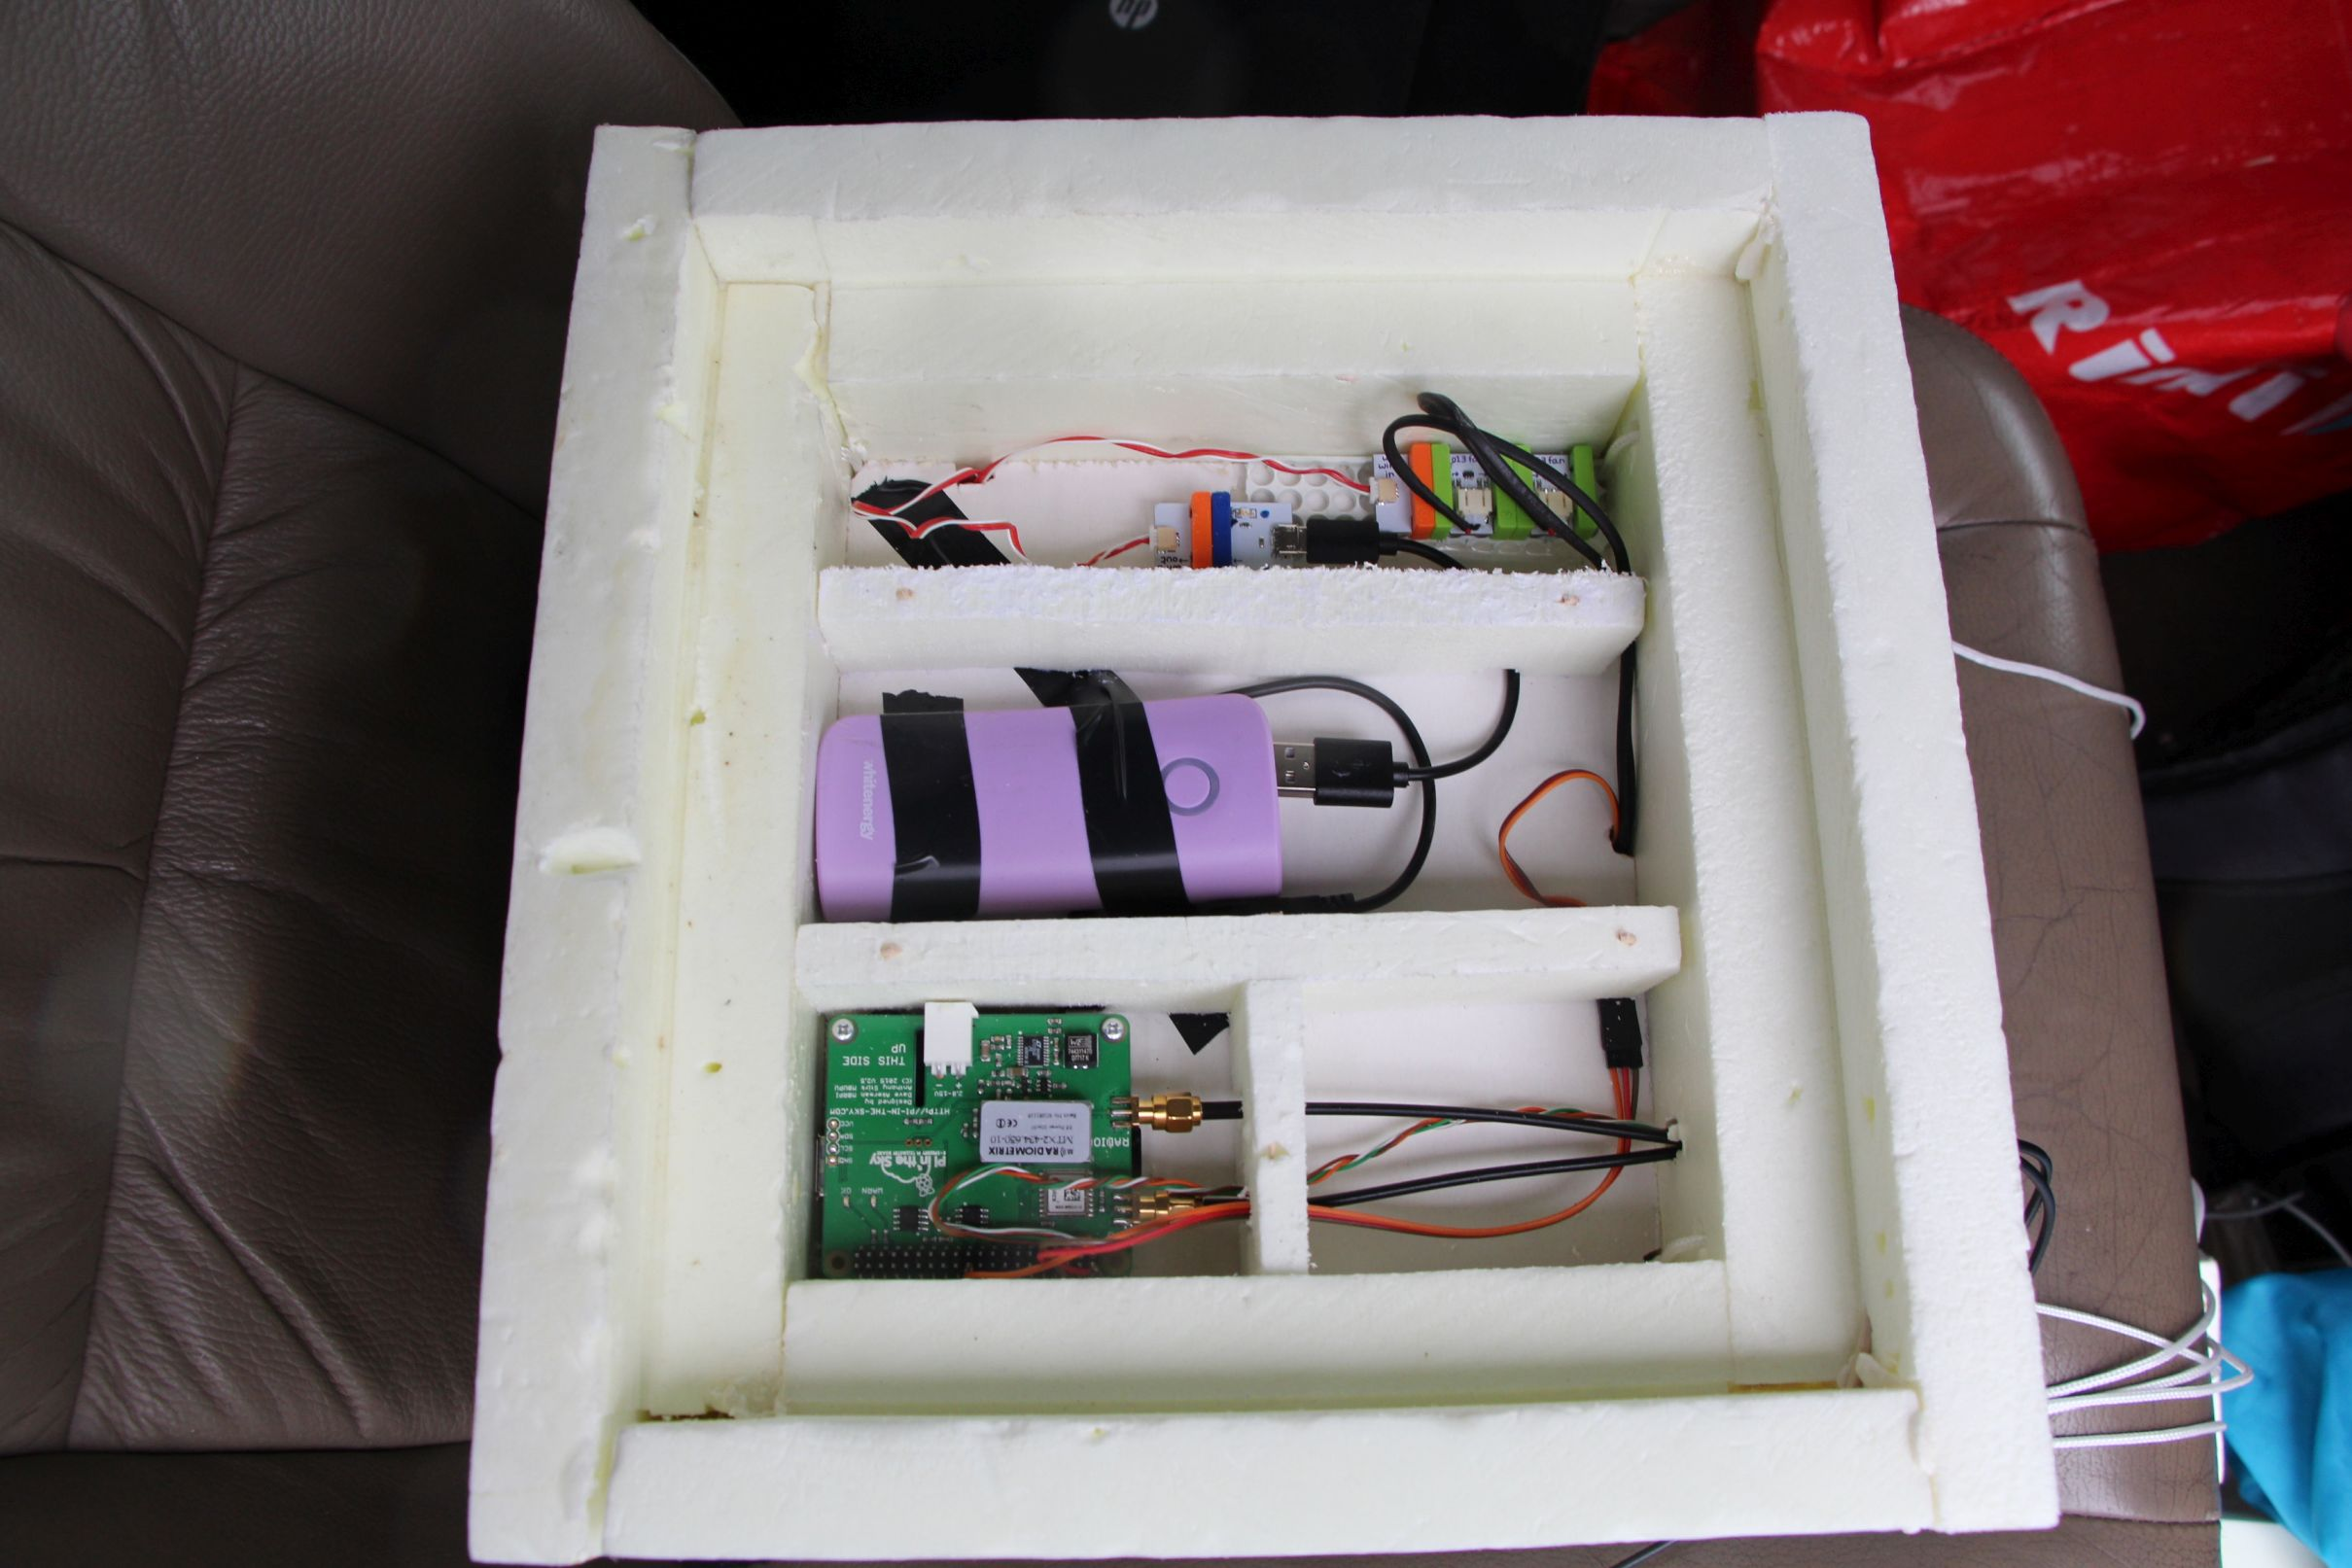
\includegraphics[width=0.5\textwidth]{PicGra/sond1korrus1.jpg}
	\caption{Pilt sondist}
	\allikas{\url{http://pildid.real.edu.ee/main.php?g2_itemId=84949}}
	\label{sond}
\end{figure}

Sondi mass oli \SI{1375}{g}. Sondi korpus oli ehitatud kasutades penoplasti ja puit tikke. Sondist tuli välja nii raadio kui ka GPS antenn, ning ka andur BME280. Sondi peale oli kinnitatud langevari. Eraldi korpuses asus GPS tracker GL370?? mida kasutatti pärast sondi leidmisel. Lennuks kasutatti Hwoyee \SI{600}{g} õhupalli.

\begin{figure}[h]
	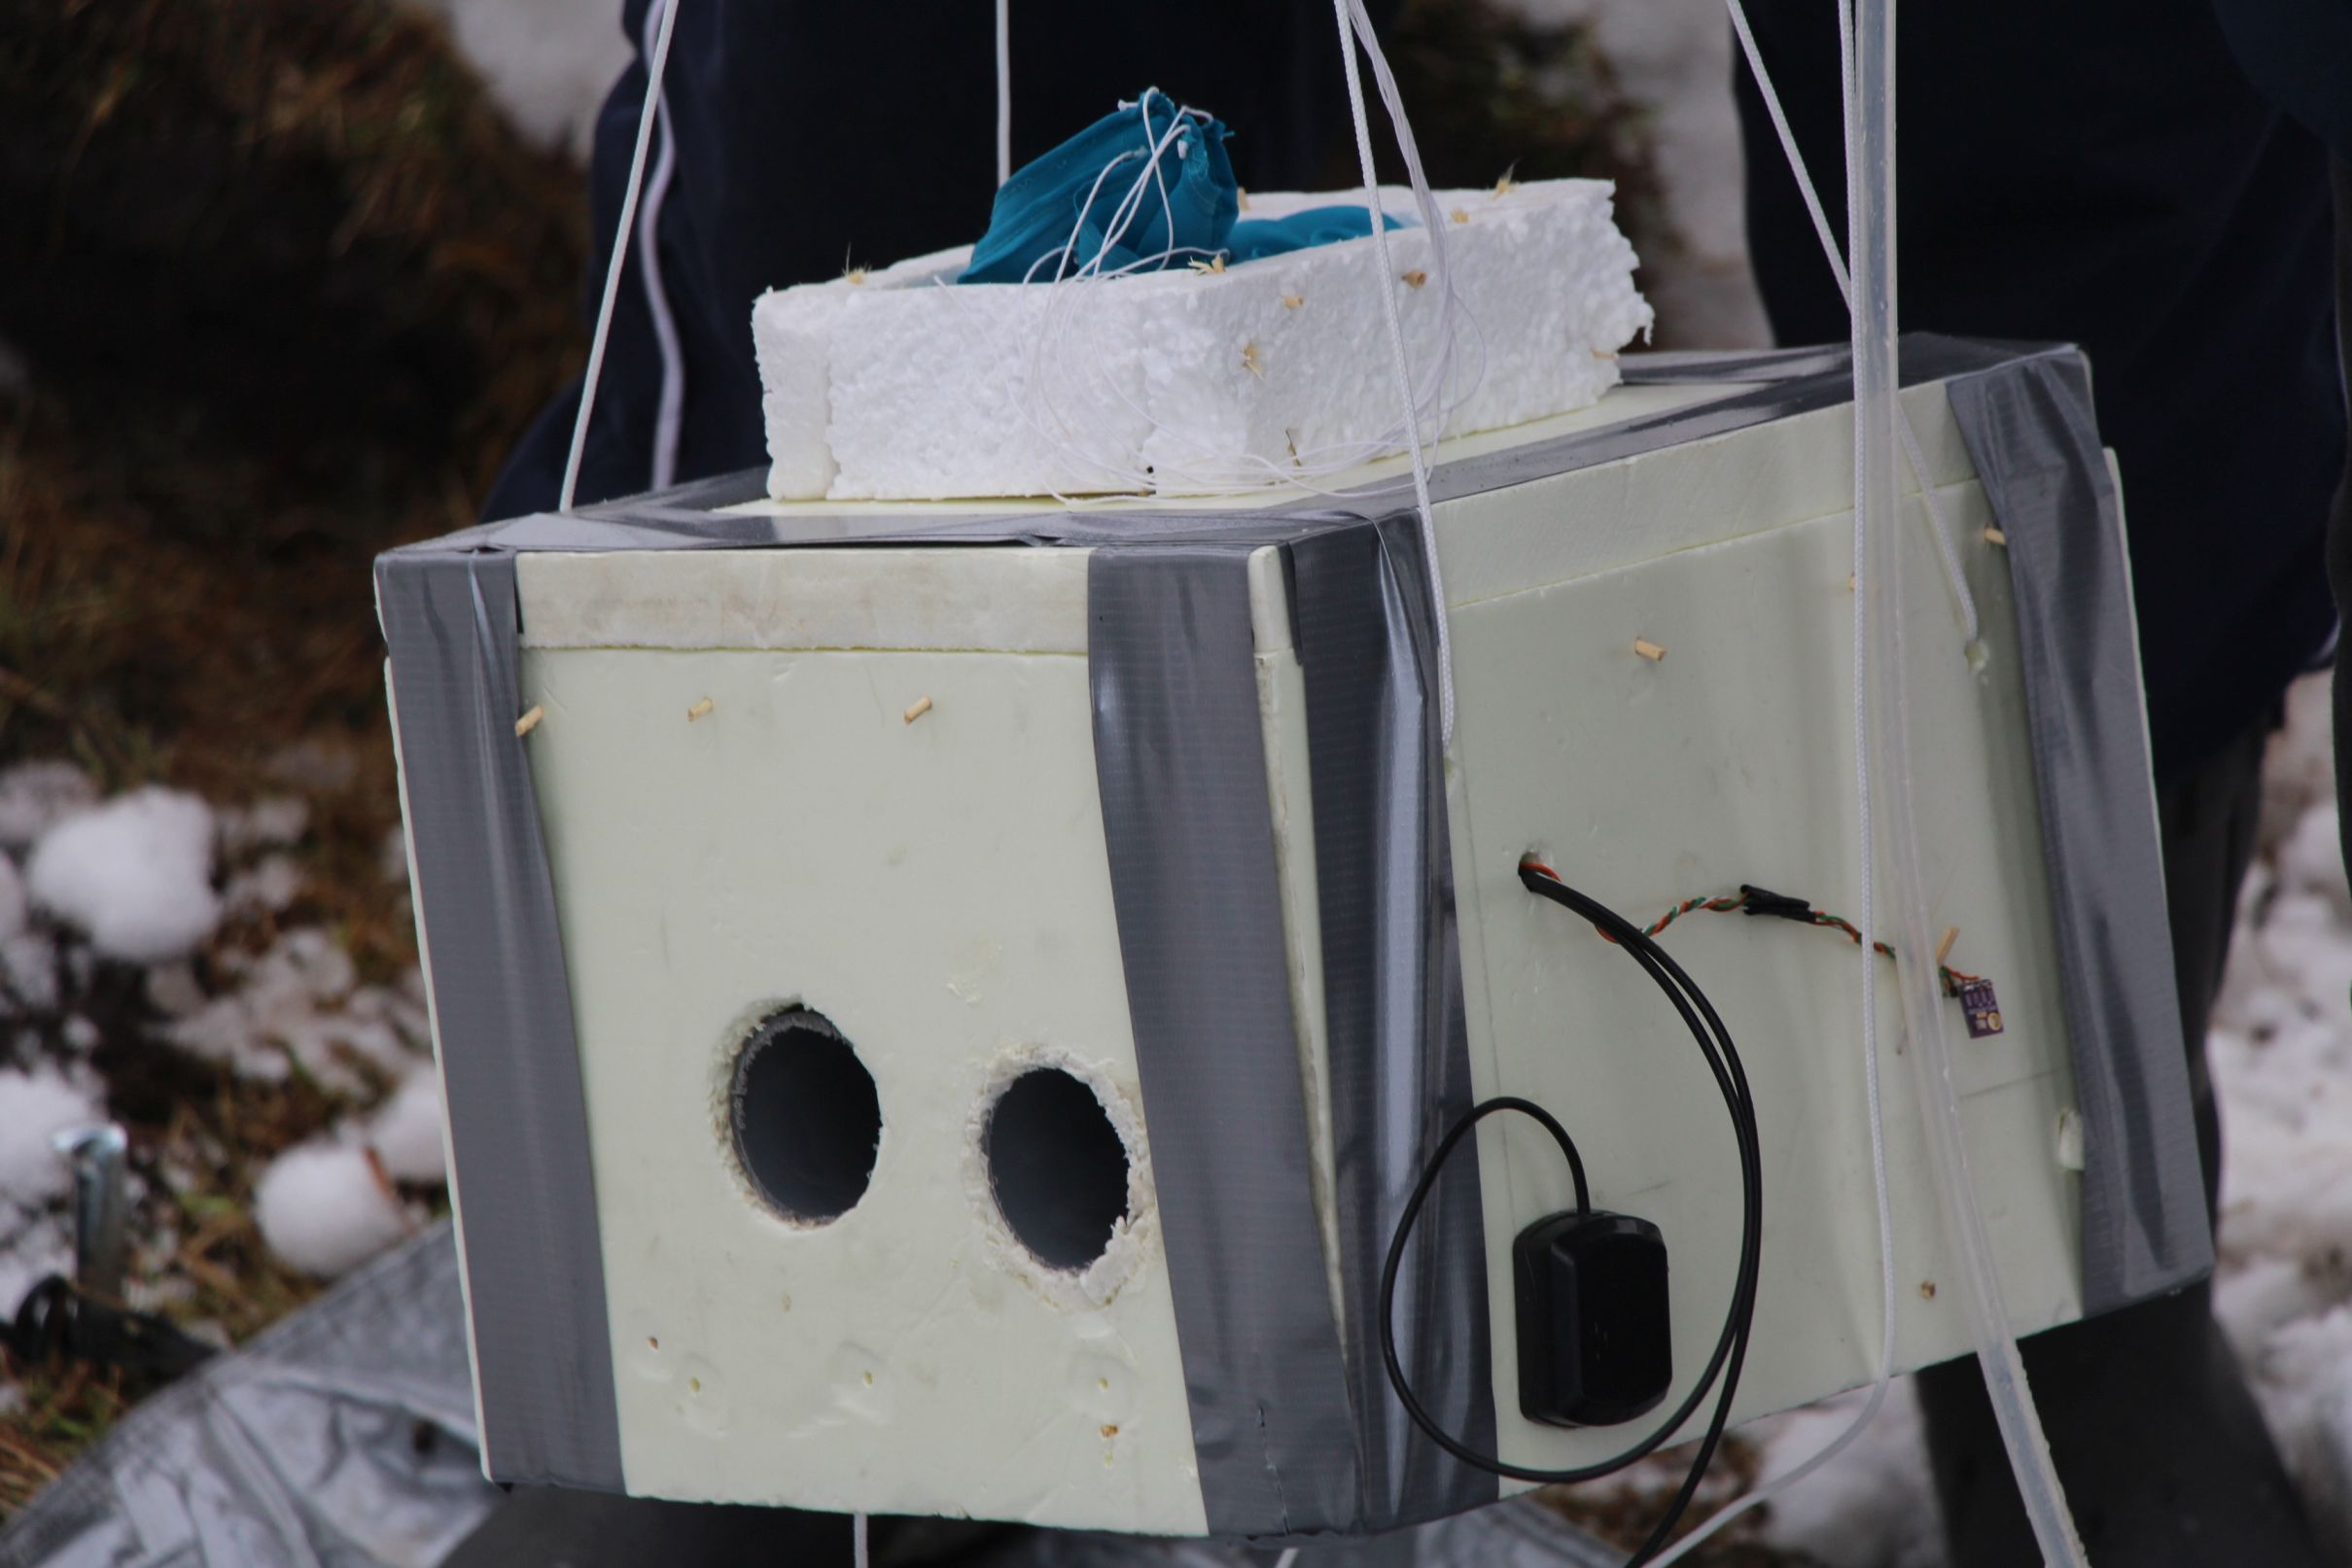
\includegraphics[width=0.5\textwidth]{PicGra/sond.jpg}
	\caption{Pilt sondist}
	\allikas{\url{http://pildid.real.edu.ee/main.php?g2_itemId=84949}}
	\label{sond}% Selle järgi viidatakse, see rida peab olema pärast \caption
\end{figure}

\subsection{Lend}

Lennu start oli kell 11:51. Algul saadi andmeid kätte raadio teel saadetud signaalist. Raadioside töötas umbes 20 min. Peale seda polnud võimalik puhast signaali kätte saada. Siis kadus GPS trackeri ühendus mobiilisideme teenuspakkujaga kõrguse pärast. Peale maandumist ühendas GPS Tracker ennast uuesti teenusepakkuja võrku ja saadi teada sondi kukkumise asukoht. Sond maandus Paide lähedal paarkümmend meetrit Tallinn-Tartu maanteest. Lend lõppes kell 14:06. Siis saime sondi kätta ja lugesime Raspberry Pi poolt tehtud logiandmed maha.



\chapter{Katseandmete analüüs}
Andmete analüüsimisks kasutan enda poolt kirjutatud c++/Python programmi. Programmiga saab joonistada graafikuid andmete põhjal ja kontrollida erinevaid seoseid.

\section{Lennu asukohaline ülevaade}

\begin{figure}[h]
	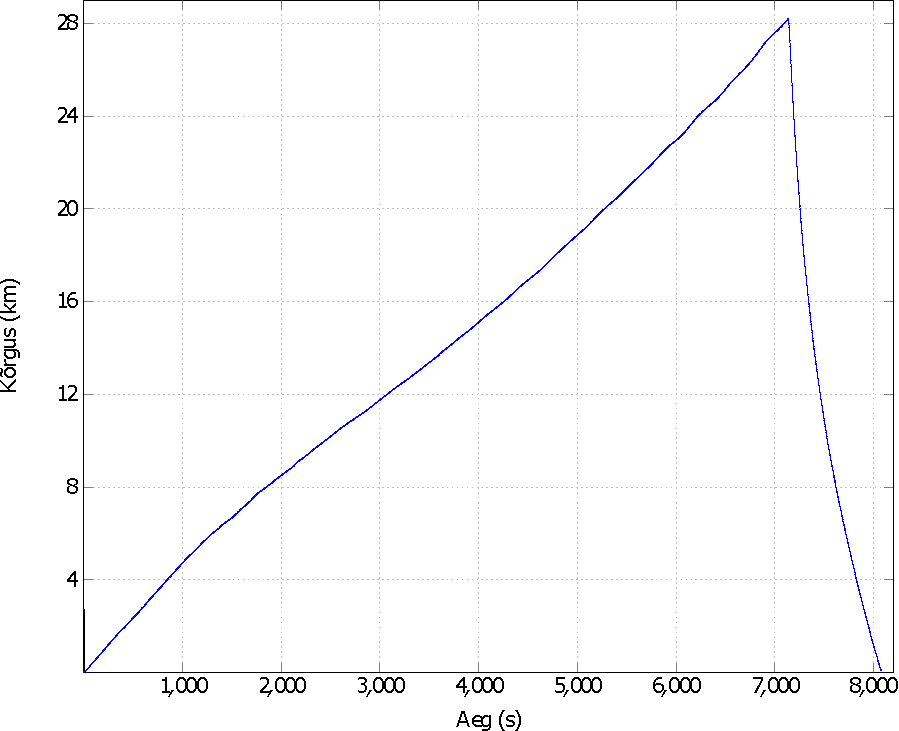
\includegraphics[width=0.5\textwidth]{PicGra/kõraeg.pdf}
	\caption{kõrguse sõltuvus ajast}
	%\allikas{Minu programm}
	\label{kõraeg}
\end{figure}

Joonisel \ref{kõraeg} on näha sondi kõrguse muutumist ajas. Kokku kestis lend \SI{8083}{s}, ehk 2 tundi, 14 min ja 43 sekundit. Selle aja jooksul tehti kokku 2460 mõõtmist. Mõõtmised on tehut sekundi tüpsuse aja tagant, eha kas iga 3 või 4 sekundi tagant. Keskmiselt tehti mõõtmisi iga \SI{3.29}{s} tagant.

Tõusmisel oli sondil ühtlane tõusukiirus. Keskmine kiirus tõustes oli \SI{3.95}{m/s}. Laskudes kiirus varieerus. Peale kukkumise algust langes sond kiiresti madala õhutihesduse tõttu. Keskmine kiirus peale langemise algust esimesel \SI{4}{km} oli \SI{78}{m/s}. Keskmine kiirus vahetult enne kokkupõrget maaga oli \SI{14}{m/s}. Kogu Kukkumise keskmine kiirus oli \SI{29.8}{m/s}.

\section{Temperatuuri muutus kõrgusega}

\begin{figure}[h]
	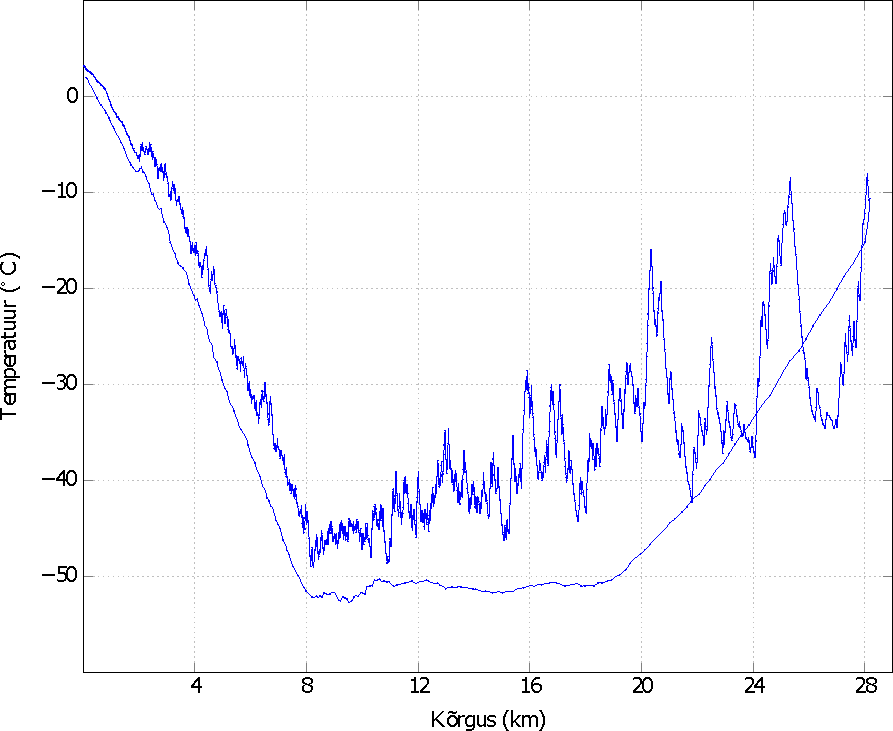
\includegraphics[width=0.5\textwidth]{PicGra/tempkõr.pdf}
	\caption{Temperatuuri sõltuvus kõrgusest}
	%\allikas{Minu programm}
	\label{TempKõrgus}% Selle järgi viidatakse, see rida peab olema pärast \caption
\end{figure}

Joonisel \ref{TempKõrgus} on näha temperatuuri muutust kõrgusega. Joonisel on kaks joont, sest andmeid mõõdeti igalt kõrguselt kaks korda, sondi tõusmisel ja sondi laskumisel. Lennu stardi ajal oli kõrgem temperatuur kui lennu lõppemise ajal.

Joonisel on näha kuidas temperatuur kõigub, mitte ei muutu ühtlaselt. See on tingitud päikese valgusest. Kui sensor on päikese poole soojendab päike sensorit. Kui sensor on sondi varjus siis peale maha jahtumist mõõdab sensor jälle tegelikku õhutemperatuuri. Sensor ei mõõda kunagi madalamat temperatuuri tegelikust õhu temperatuurist. Kõrguse kasvades muutub temperatuuri kõikumine amplituud kõrgemaks. See on tingitud madalst rõhust. Kuna õhk hõreneb hakkab sondi temperatuuri rohkem mõjutama päike kui õhk ise.

Kukkumine hakkab sel hetkel kui sensor on ülesse soojenenud. Seega sensor kukkumise ajal jahtub, kuid kuna nende kõrguste juures kõrguse langemisel langeb ka temperatuur, ei saavuta sensor välisemperatuuri, varem kui \SI{20}{km} kõrgusel maast. Sel ajal on näha sujuvat temperatuuri muutust. Sensori mitte üles soojenemist kukkumisel võib põhjendada mittut moodi. Sond võis kukkumisel hakkata tugevalt pöörlema (MIS SIIS???). Kogu lennu vältel oli sond külgtuultega samas kiiruse taustsüsteemis. Seega sondile mõjustid tuuled mis tulevad üles liikumisest ja alla kukkumisest. Kuna kuni \SI{20}{km}'ni kukkus sond keskmise kiirusega \SI{70}{m/s} siis jahutas tuul sensorit.

Kuna selles uurimistöös uuritakse täpsemalt tropsfääri osa siis võib algul välja jätta kõik muu peale esimese umbes \SI{8}{km}. Täpseks kõrguseks valiti \SI{8154}{m}. Sellel kõrgusel tehti viimane mõõtmine mis oli temperatuurigraafiku viimane lokaalne miinimum peale mida hakkas temperatuur jälle tõusma. Kuna graafik on ebatasane vastab lokaalne miinimum kõige paremini tegelikkule temperatuurile. Sama kõrgus valiti ka kukkumisel. Tõusmisel on selles vahemikus \SI{578} andmepunkti ja laskumisel on selles vahemikus \SI{144} andmepunkti.

\begin{figure}[h]
	\includegraphics[width=0.5\textwidth]{PicGra/tempkõrtrop.pdf}
	\caption{Temperatuuri sõltuvus kõrgusest alla \SI{8}{km}}
	\allikas{Autori erakogu}
	\label{tempkõrtrop}% Selle järgi viidatakse, see rida peab olema pärast \caption
\end{figure}

Jooniselt \ref{tempkõrtrop} märgati anomaaliat. Umbes \SI{2}{km} kõrgusel on nii laskumisel kui ka tõusmisel näha kõrguse tõusmisega väikest temperatuuri muutust. Kuna see toimub nii tõusmisel kui ka kukkumisel siis on see suure tõenäelsusega tegelik temperatuuri muutus ja mitte sensori viga või muud sellist.

\begin{figure}[h]
	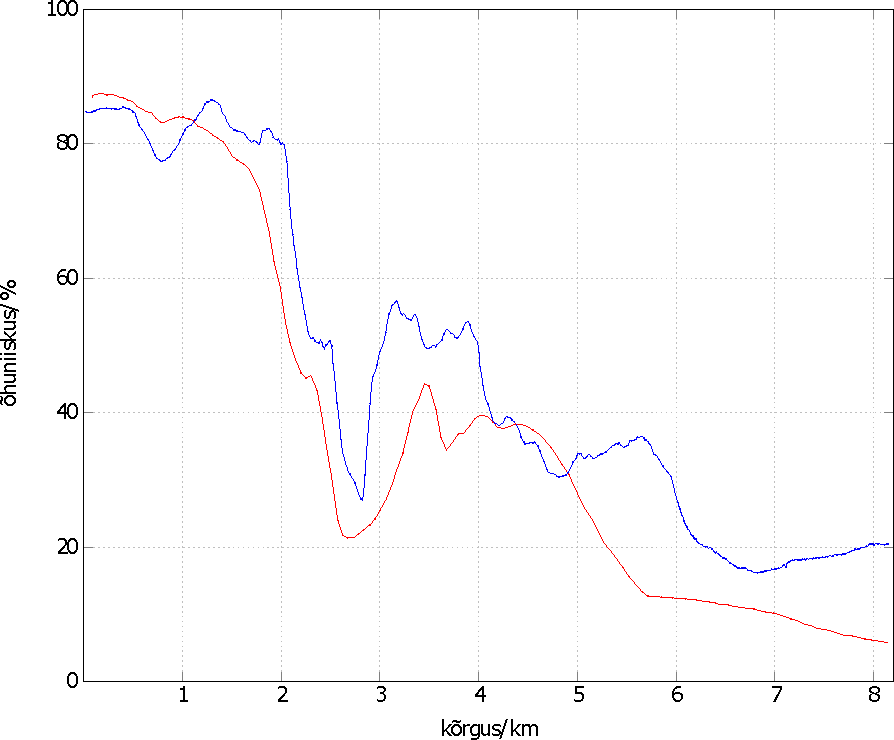
\includegraphics[width=0.5\textwidth]{PicGra/humkõrtrop.pdf}
	\caption{õhuniisekuse sõltuvus kõrgusest alla \SI{8}{km}}
	\allikas{Autori erakogu}
	\label{humkõrtrop}% Selle järgi viidatakse, see rida peab olema pärast \caption
\end{figure}

Vaadates joonist \ref{humkõrtrop} on näha, et kuni \SI{2}{km} kõrguseni on õhuniiskus ühtlselt kõrge. Kuid peale \SI{2}{km} on näha, et õhuniiskus langeb tugevalt. Õhuniiskus langes, kuna sond väljus pilvedest, ning temperatuur tõusis. Pilvedest väljumist saab ka tõestada temperatuuri kõikumise algusega. Kuni \SI{2}{km}'ni temperatuur ei kõikunud, kuna päikest ei paistnud sondile peale. Pilvedest väljudes hakkas aga päike mõjutama sensori lugemist. Kuna osa mõõtmisi tehti pilvede sees ja osa pilvedest väljas otsustatti vaadelda temperatuuri muutumist eraldi pilvede sees ja pilvedest väljas.

\subsection{temperatuuri muutus kõrgusega pilvedes sees ja allpool}
Pilvede sees vaadati temperatuure tõustes kuni  \SI{2010}{m} meetrini. Sellel kõrgusel tehti viimane mõõtmine peale mida temperatuur tõusis pilvedest väljumise tagajärgel. Samal põhjusel valiti laskumisel viimaseks andmepunktiks \SI{1926}{m} kõrgusel mõõdetud andmepunkt. Sellel kõrgusvahemikul teht tõustes \SI{133} mõõtmist ja langedes \SI{41} mõõtmist.

\begin{figure}[h]
	\includegraphics[width=0.5\textwidth]{PicGra/tempkõrtroppilvlin.pdf}
	\caption{temperatuuri sõltuvus kõrgusest alla \SI{2}{km}}
	\allikas{Autori erakogu}
	\label{tempkõrtroppilvlin}% Selle järgi viidatakse, see rida peab olema pärast \caption
\end{figure}

Joonisel \ref{tempkõrtroppilvlin} on graafikutele sobitatud võimalikult täpne lineaarne seos kõrguse ja temperatuuri vahel. Parima seose puhul tõusmisel muutub temperatuur \SI{-5.04572}{\degreeCelsius/km} ja algtemperatuur kõrgusel \SI{0}{m} merepinnast on \SI{3.98954}{\celsius} $r=-0.9929$. Laskumisel muutub temperatuur \SI{-5.53009}{\degreeCelsius/km} ja algtemperatuur kõrgusel \SI{0}{m} merepinnast on \SI{2.61829}{\celsius} $r=-0.999$.


\subsection{temperatuuri muutus kõrgusega pilvedest kõrgemal}
Tõusmisel valiti algpunktiks \SI{2565}{m} kõrgusel mõõdetud andmepunkt. See on esimene andmepunkt,alates \SI{2010}{m} kõrgusel asuvast andmepunktist, kus on madalam temperatuu kui \SI{2010}{m} kõrgusel mõõdetud temperatuur.

Laskumisel valiti algpunktiks \SI{2136}{m} kõrgusel mõõdetud andmepunkt. See on esimene andmepunkt, alates \SI{1926}{m} kõrgusel mõõdetud andmepunktist, kus on madalam temperatuu kui \SI{1926}{m} kõrgusel mõõdetud temperatuur.

\begin{figure}[h]
	\includegraphics[width=0.5\textwidth]{PicGra/tempkõrtroplin.pdf}
	\caption{temperatuuri sõltuvus kõrgusest üle \SI{2}{km}}
	\allikas{Autori erakogu}
	\label{tempkõrtroplin}% Selle järgi viidatakse, see rida peab olema pärast \caption
\end{figure}


Joonisel \ref{tempkõrtroplin} on graafikutele sobitatud võimalikult täpne lineaarne seos kõrguse ja temperatuuri vahel. Parima seose puhul tõusmisel muutub temperatuur \SI{-7.13398}{\degreeCelsius/km} ja algtemperatuur kõrgusel \SI{0}{m} merepinnast on \SI{12.8454}{\celsius} $r=-0.9951$. Laskumisel muutub temperatuur \SI{-7.67992}{\degreeCelsius/km} ja algtemperatuur kõrgusel \SI{0}{m} merepinnast on \SI{9.13797}{\celsius} $r=-0.9994$.

Tõusmise graafik on kõikuv mille on põhjustanud päike. Kuna päike soojendas siis sensor mõõtis tegelikust kõrgemat temperatuuri. Kui sensor jahtus siis mõõtis sensor tegelikku temperatuuri. Kindlasti ei mõõtnud sensor tegelikkust madalamat temperatuuri. Kasutades seda asjaolu võib eemaldada kõik hüpplevad kohad. Andmeid hakkati madalama kõrgusega alates vaatama nii, et temperatuur pidevalt langeks. Kui kõrguse tõusetes temperatuur tõuseb eemaltatti järjest kõik andmepunktid kuni jõuti andmepunktini mis oli madalam viimasest võrdluspunktist.

\begin{figure}[h]
	\includegraphics[width=0.5\textwidth]{PicGra/tempkõrtroplinstalin.pdf}
 	\caption{temperatuuri sõltuvus kõrgusest üle \SI{2}{km}}
 	\allikas{Autori erakogu}
 	\label{tempkõrtroplinstalin}% Selle järgi viidatakse, see rida peab olema pärast \caption
\end{figure}

Joonisel \ref{tempkõrtroplinstalin} on graafikutele sobitatud võimalikult täpne lineaarne seos kõrguse ja temperatuuri vahel. Parima seose puhul tõusmisel muutub temperatuur \SI{-7.23193}{\degreeCelsius/km} ja algtemperatuur kõrgusel \SI{0}{m} merepinnast on \SI{12.5889}{\celsius} $r=-0.998$.











\addchap{Kasutatud materjalid}% Viitamine paraneb veel

Hobbs, P. V., Wallace, J. M. (2006) Atmospheric Science: An Introductory Survey. Amsterdam: Elsevier \newline
Ahrens, C. D., Henson, R. (2018) Meteorology Today: An Introduction to Weather, Climate, and the Environment. Boston: Cengage Learning

%\cite{examplebook}% Kõige lihtsam viitamise käsk 
%\cite{examplearticle}
%\cite{exampleonline}

%\printbibliography% Selle käsuga trükime kasutatud materjalid, kommenteeri see kiirema kompileerimise jaoks

%\appendix% Lisad
%\chapter{Kes see lisatööd ikka teha tahab}% Lisa pealkiri

\kinnitusleht% Kinnitusleht
\end{document}
